\section{Query, Key, Value (QKV)}
\begin{frame}{Query, Key, Value (QKV)}
  \begin{itemize}
    \item[$\blacktriangleright$] \textbf{Query:} What you want (the search)
    \item[$\blacktriangleright$] \textbf{Key:} Index of content (where to look)
    \item[$\blacktriangleright$] \textbf{Value:} Actual content (what you get)
  \end{itemize}
  \vspace{1em}
  \textit{Intuition}
  \begin{itemize}
    \item[] Think of QKV like a search engine:
    \begin{itemize}
      \item[$\blacktriangleright$] \textbf{Query (Q):} Comes from the current decoder state (or token)
      \item[$\blacktriangleright$] \textbf{Key (K)}, \textbf{Value (V):} Come from the encoder (or input sequence)
    \end{itemize}
  \end{itemize}
\end{frame}

\begin{frame}{QKV -- Formulation}
\textbf{Given:}
\begin{itemize}
    \item[$\blacktriangleright$] Input sequence $\mathbf{X}$
\end{itemize}
\vspace{0.5em}
\textbf{Linear projections:}
\begin{align*}
    \mathbf{Q} &= \mathbf{X} W_Q \\
    \mathbf{K} &= \mathbf{X} W_K \\
    \mathbf{V} &= \mathbf{X} W_V \\
\end{align*}

\vspace{0.5em}
\textbf{Attention:} score $\mathbf{Q}$ against $\mathbf{K}$ with the scaled dot-product alignment, softmax the scores, and take the weighted sum of $\mathbf{V}$.
\end{frame}

\begin{frame}{Query, Key, Value (QKV)}
  \centering
  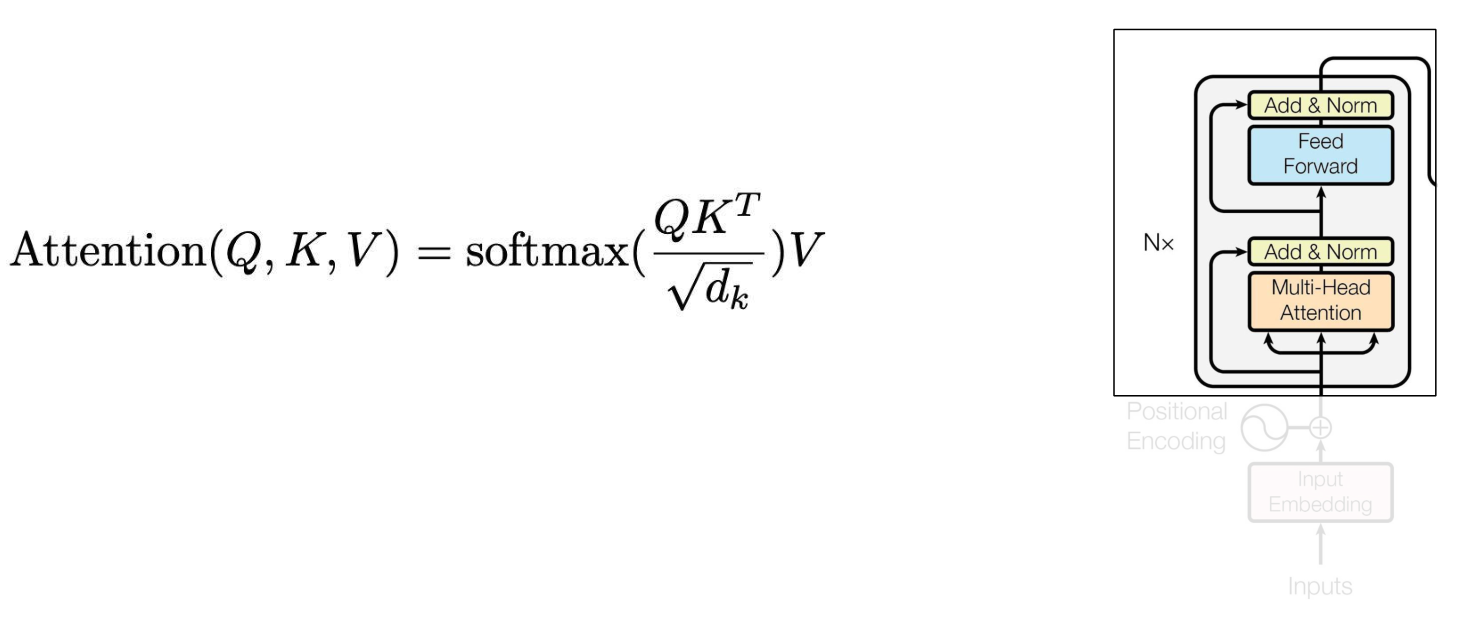
\includegraphics[width=0.7\paperwidth,height=0.66\paperheight,keepaspectratio]{images/attention-deep-dive/attention_qkv_formula_transformer.png}

  {\scriptsize Source: CMU 11-785 (Spring 2024), Lecture 19: Transformers and Newer Architectures, slide~33.}
\end{frame}

\begin{frame}{Query, Key, Value (QKV)}
  \centering
  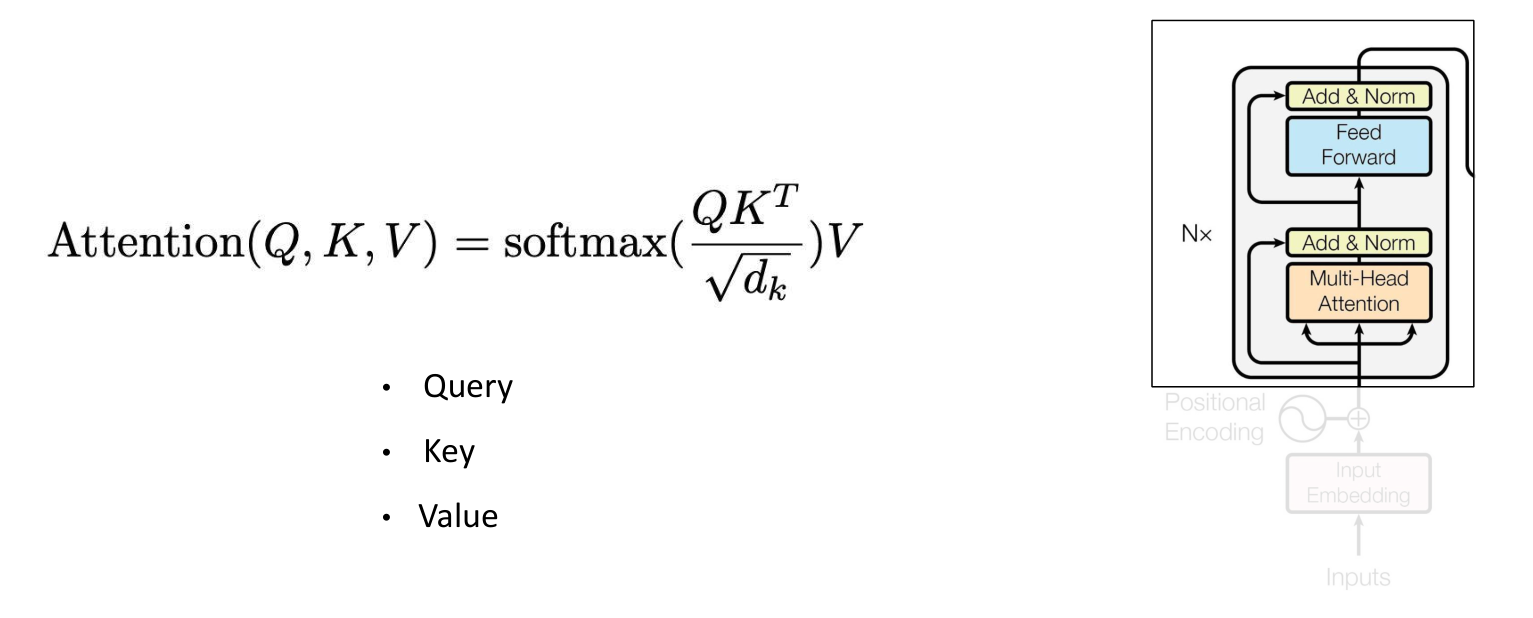
\includegraphics[width=0.7\paperwidth,height=0.66\paperheight,keepaspectratio]{images/attention-deep-dive/attention_qkv_formula_query_key_value.png}

  {\scriptsize Source: CMU 11-785 (Spring 2024), Lecture 19: Transformers and Newer Architectures, slide~34.}
\end{frame}

\begin{frame}{Query, Key, Value (QKV)}
  \centering
  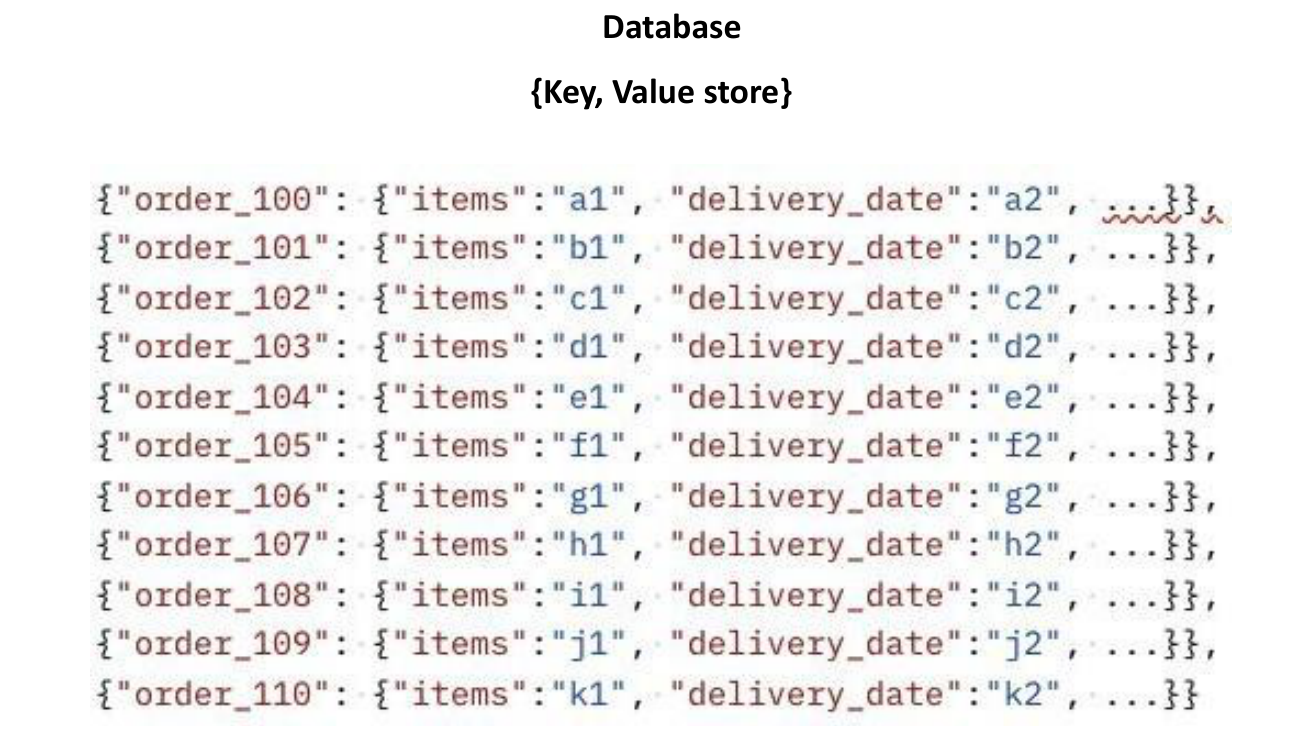
\includegraphics[width=0.7\paperwidth,height=0.66\paperheight,keepaspectratio]{images/attention-deep-dive/attention_database_key_value_store.png}

  {\scriptsize Source: CMU 11-785 (Spring 2024), Lecture 19: Transformers and Newer Architectures, slide~35.}
\end{frame}

\begin{frame}{Query, Key, Value (QKV)}
  \centering
  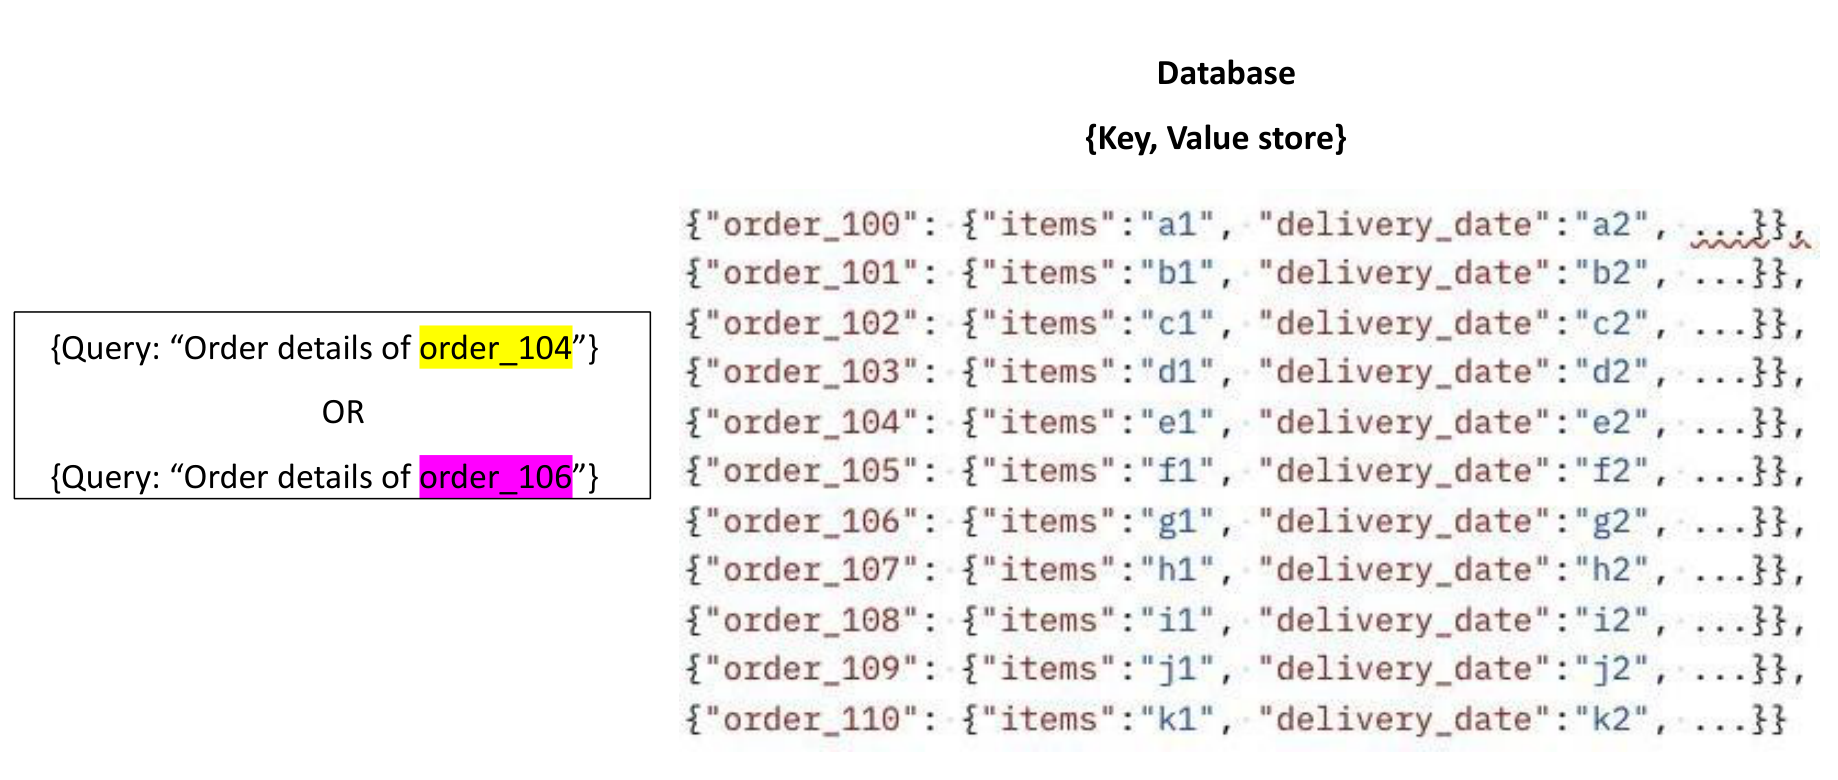
\includegraphics[width=0.7\paperwidth,height=0.66\paperheight,keepaspectratio]{images/attention-deep-dive/attention_database_query_lookup.png}

  {\scriptsize Source: CMU 11-785 (Spring 2024), Lecture 19: Transformers and Newer Architectures, slide~36.}
\end{frame}

\begin{frame}{Query, Key, Value (QKV)}
  \centering
  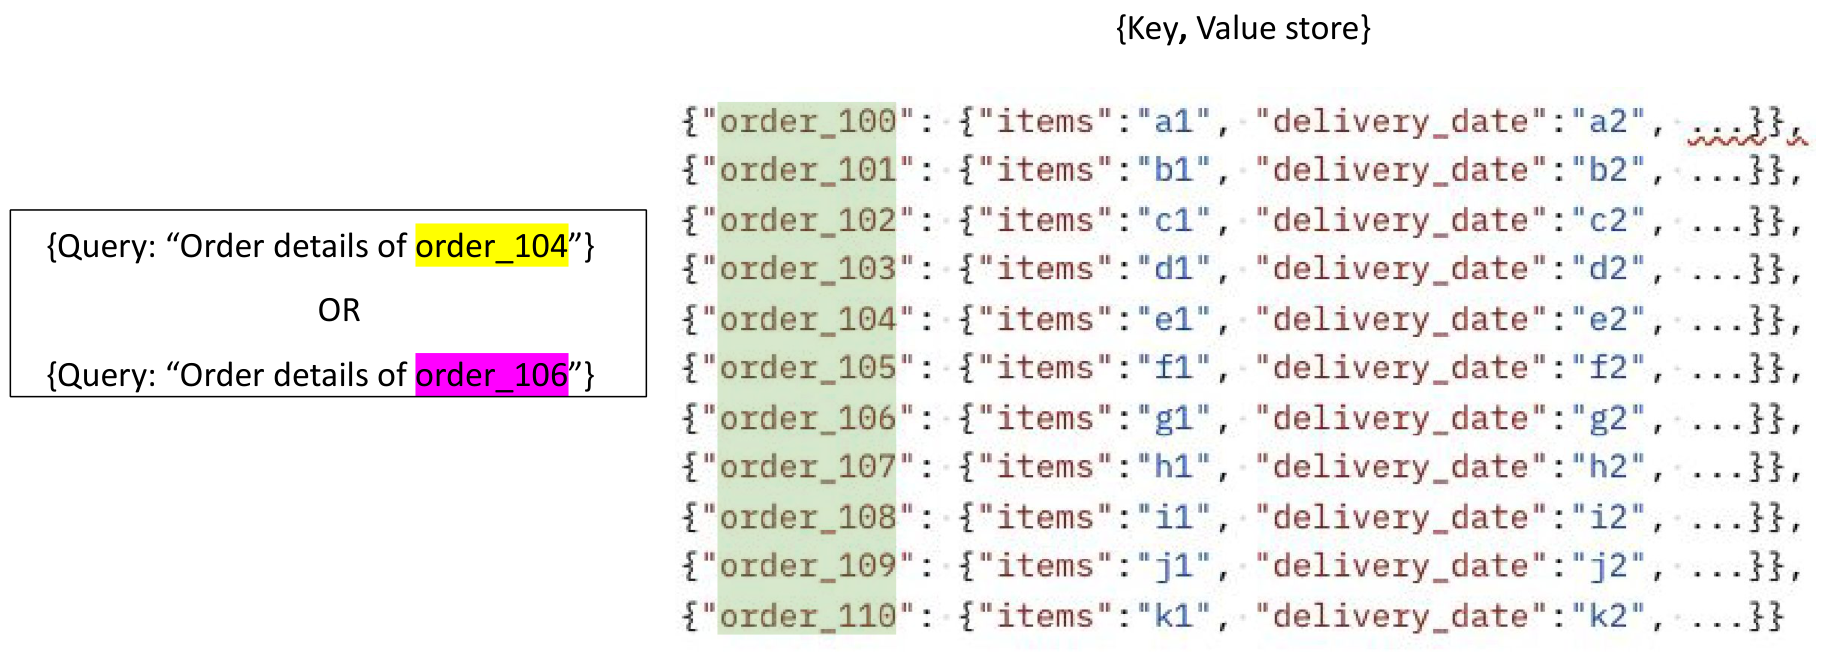
\includegraphics[width=0.7\paperwidth,height=0.66\paperheight,keepaspectratio]{images/attention-deep-dive/attention_database_query_matches.png}

  {\scriptsize Source: CMU 11-785 (Spring 2024), Lecture 19: Transformers and Newer Architectures, slide~37.}
\end{frame}

\begin{frame}{Query, Key, Value (QKV)}
  \centering
  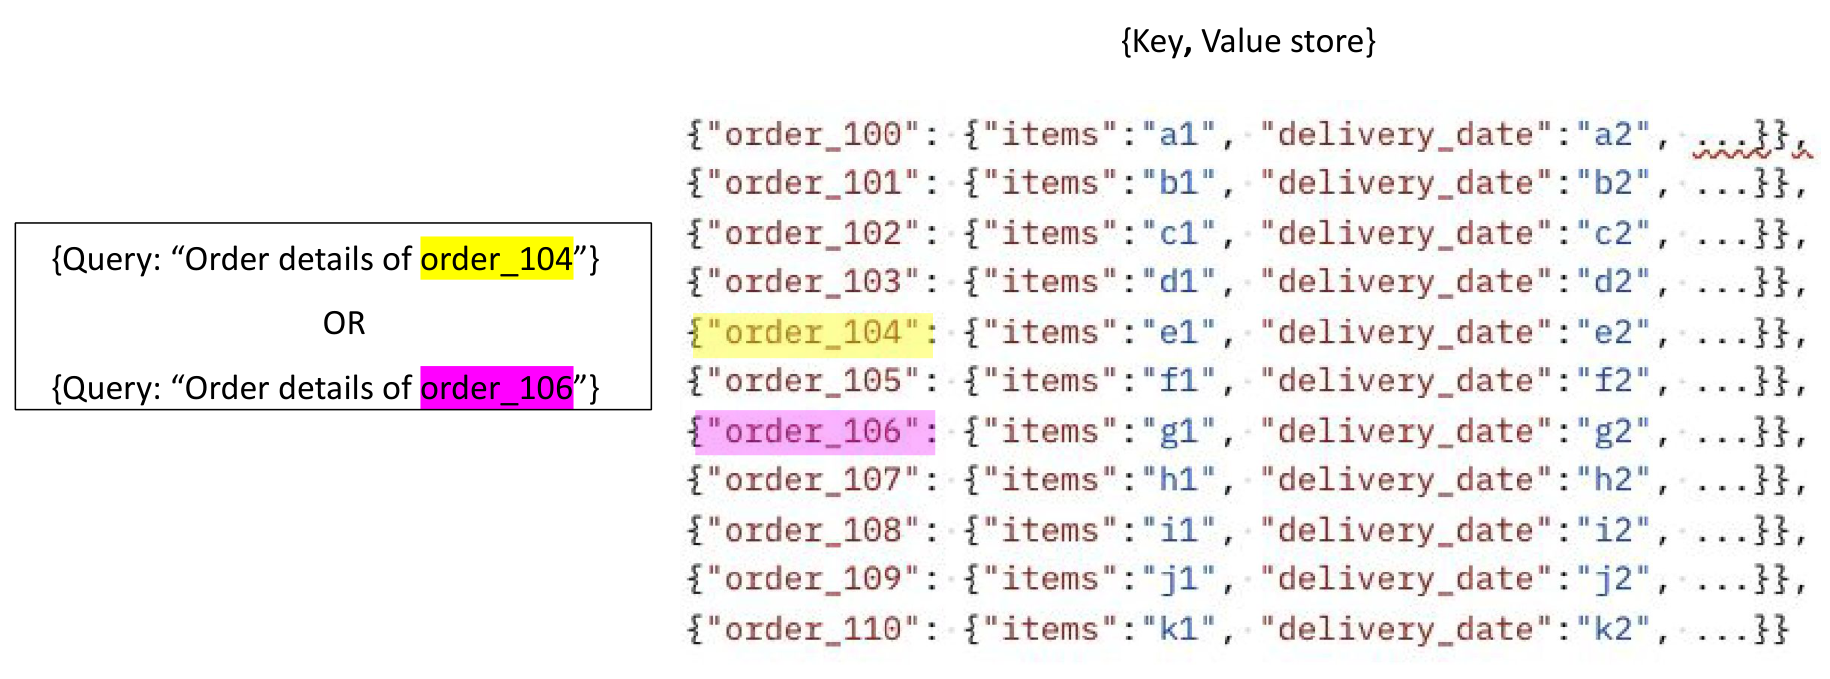
\includegraphics[width=0.7\paperwidth,height=0.66\paperheight,keepaspectratio]{images/attention-deep-dive/attention_database_two_queries.png}

  {\scriptsize Source: CMU 11-785 (Spring 2024), Lecture 19: Transformers and Newer Architectures, slide~38.}
\end{frame}

\begin{frame}{Query, Key, Value (QKV)}
  \centering
  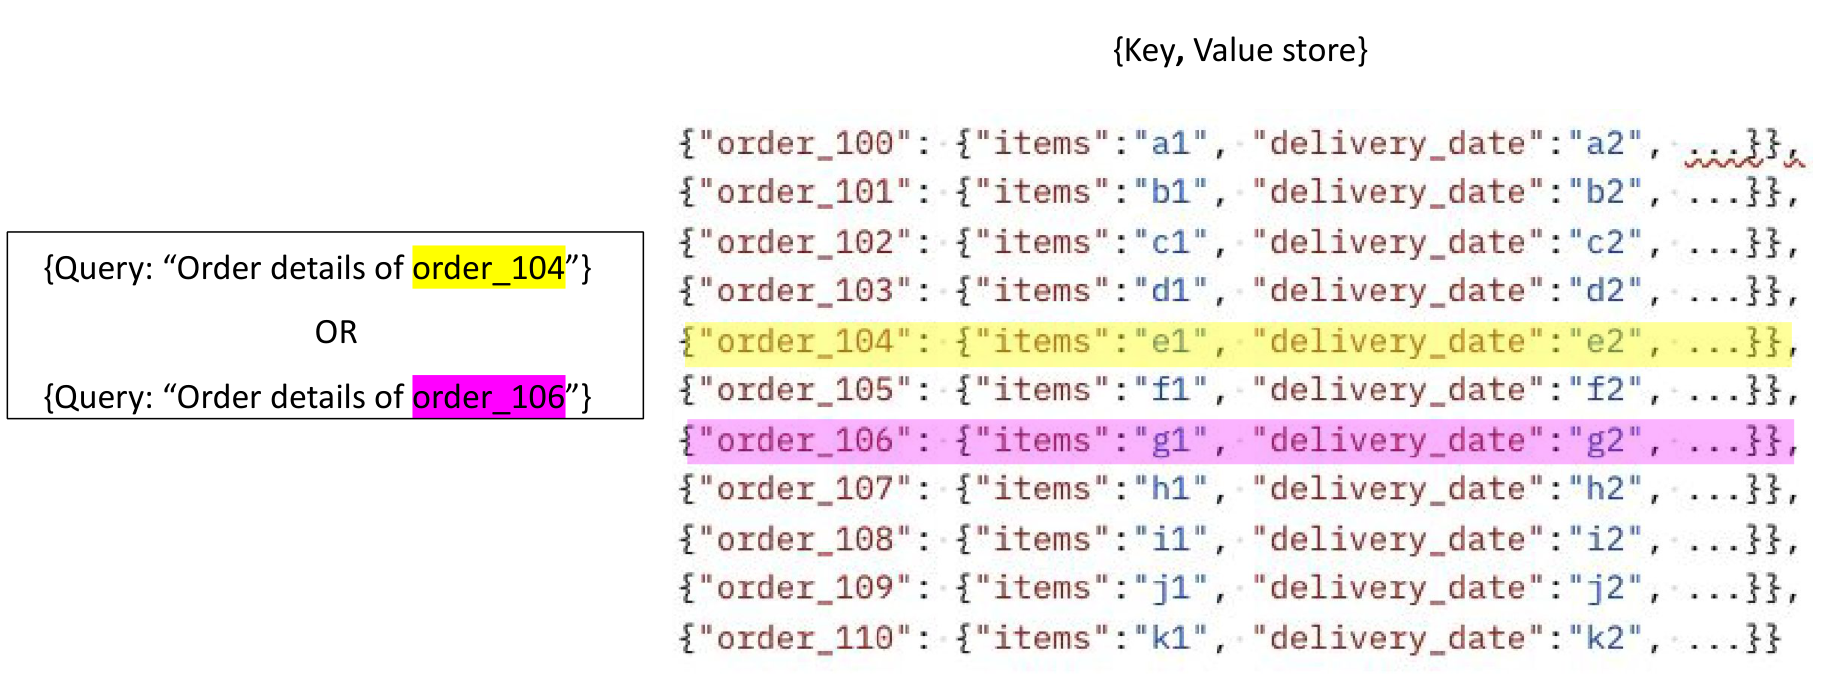
\includegraphics[width=0.7\paperwidth,height=0.66\paperheight,keepaspectratio]{images/attention-deep-dive/attention_database_two_matches_highlighted.png}

  {\scriptsize Source: CMU 11-785 (Spring 2024), Lecture 19: Transformers and Newer Architectures, slide~39.}
\end{frame}

\begin{frame}{Query, Key, Value (QKV)}
  \centering
  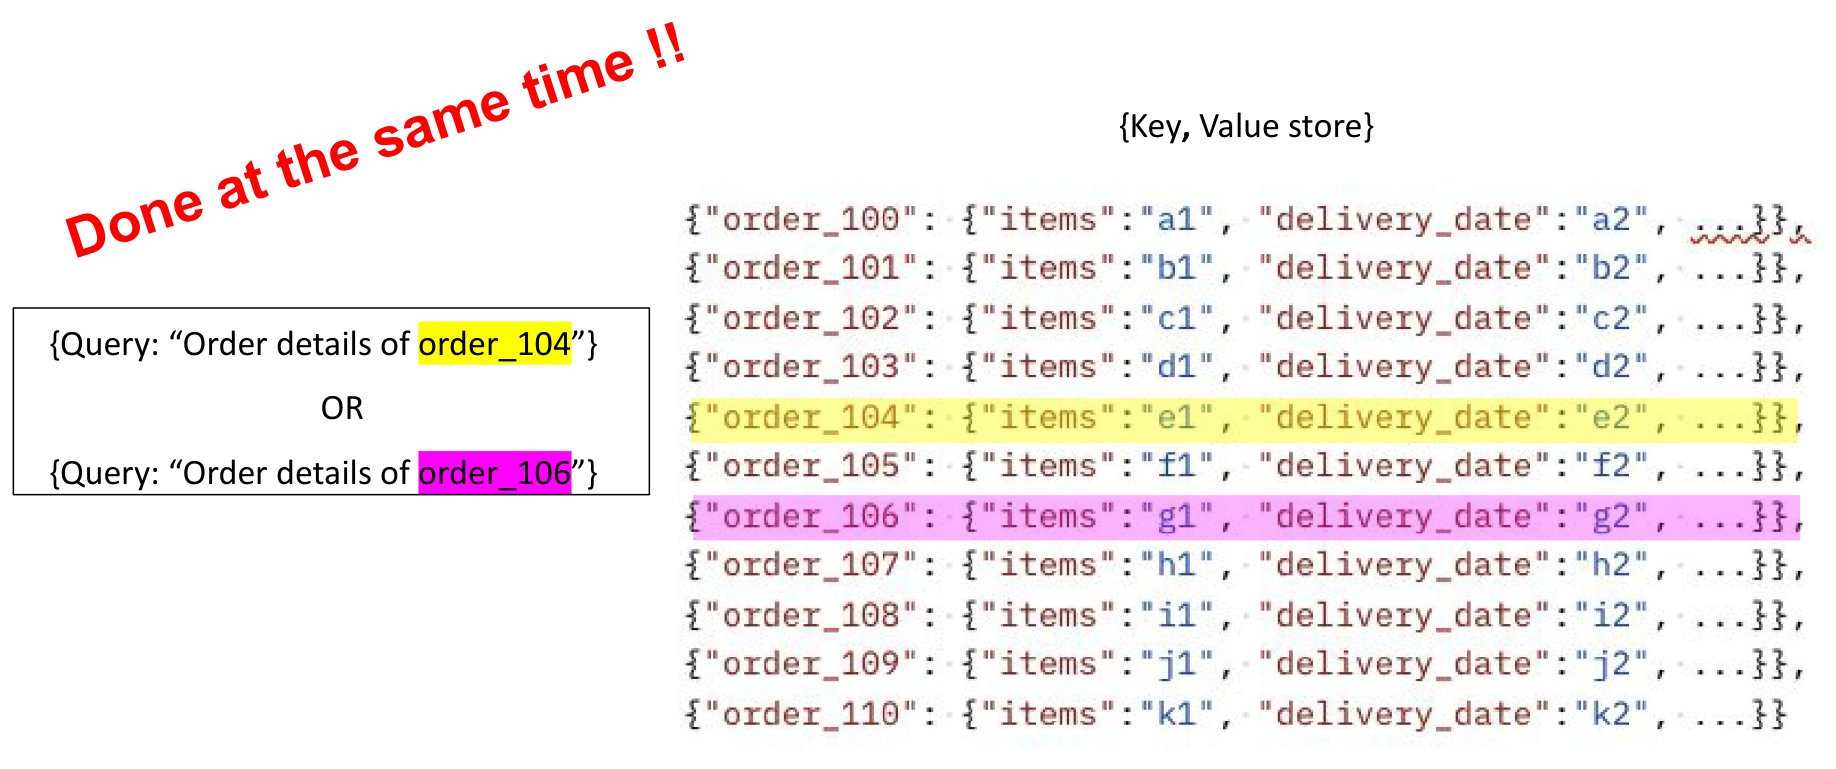
\includegraphics[width=0.7\paperwidth,height=0.66\paperheight,keepaspectratio]{images/attention-deep-dive/attention_database_parallel_lookup.png}

  {\scriptsize Source: CMU 11-785 (Spring 2024), Lecture 19: Transformers and Newer Architectures, slide~40.}
\end{frame}

\begin{frame}{Query, Key, Value (QKV)}
  \centering
  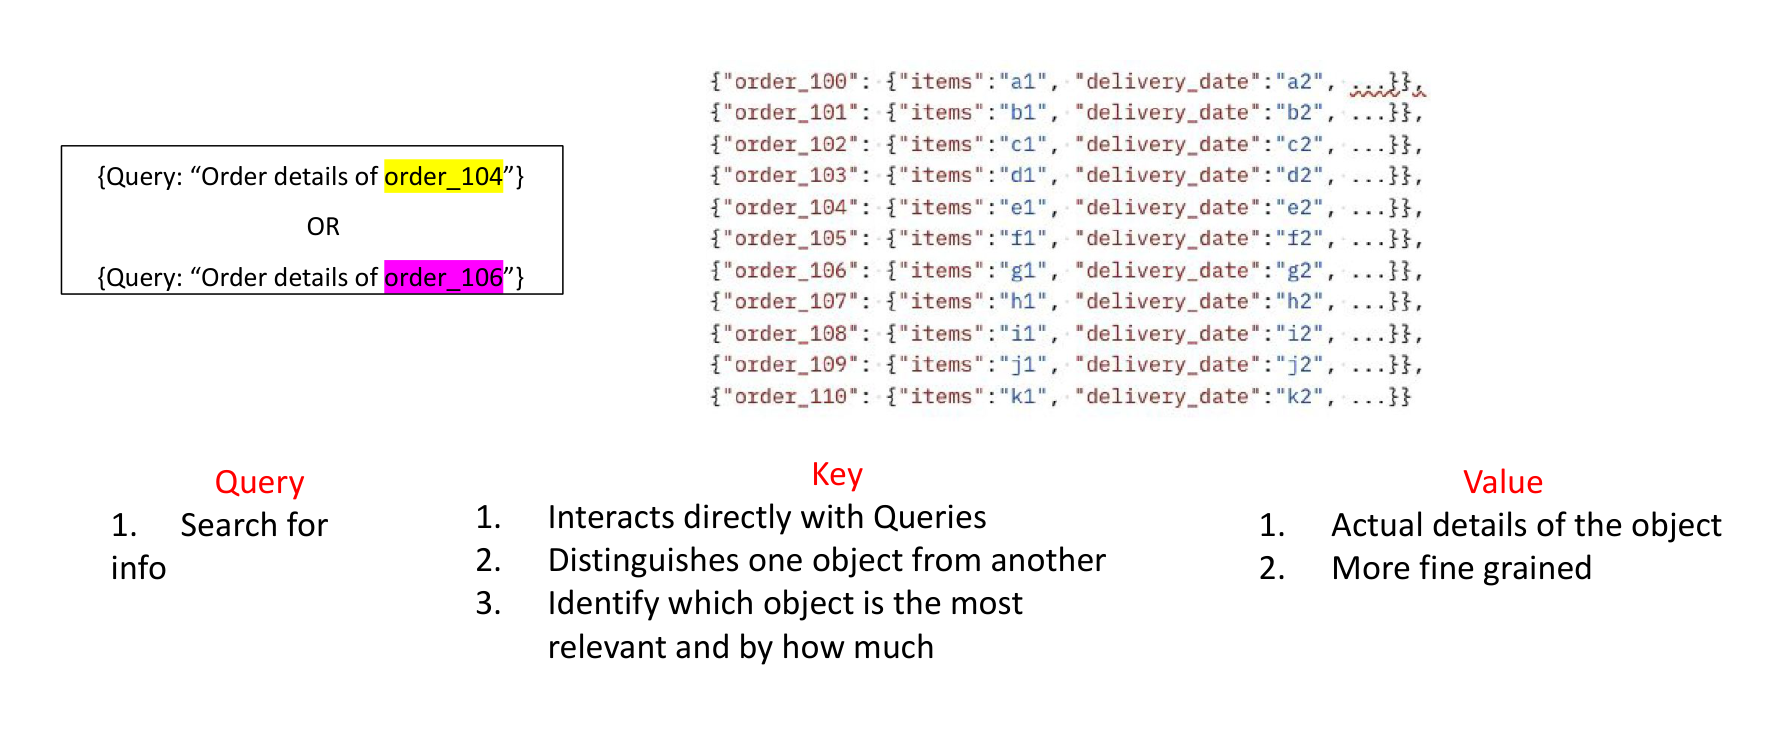
\includegraphics[width=0.7\paperwidth,height=0.66\paperheight,keepaspectratio]{images/attention-deep-dive/attention_qkv_roles_summary.png}

  {\scriptsize Source: CMU 11-785 (Spring 2024), Lecture 19: Transformers and Newer Architectures, slide~41.}
\end{frame}
